%%%%%%%%%%%%%%%%%%%%%%%%%%%%%%%%%%%%%%%%%%%%%%%%%%%%%%%%%%%%
%% Capítulo 1 / Introducción
%%%%%%%%%%%%%%%%%%%%%%%%%%%%%%%%%%%%%%%%%%%%%%%%%%%%%%%%%%%%
\chapter{Introducción}
\epigrafe{Everyone in this country should learn how to program a computer, because it teaches you how to think.}
              {\textsc{Steve Jobs}}

\textcolor{gray}{Es el contenido global de lo que va a encontrarse en el trabajo. Incluye los aspectos relevantes de los antecedentes, la definición del problema, la justificación, los objetivos: general y específicos. En este apartado se iniciará la paginación principal con números arábigos (los capítulos podrán ir numerados con arábigos)}

%%%%%%%%%%%%%%%%%%%%%%%%%%%%%%%%%%%%%%%%%%%%%%%%%%%%%%%%%%%%
\section{Ejemplo Figura}
\lipsum[1] 
Como se puede apreciar en la Figura \ref{fig:01_Proceso}.

\begin{figure}[htbp]                                                      % Inclusión de una figura
\centering
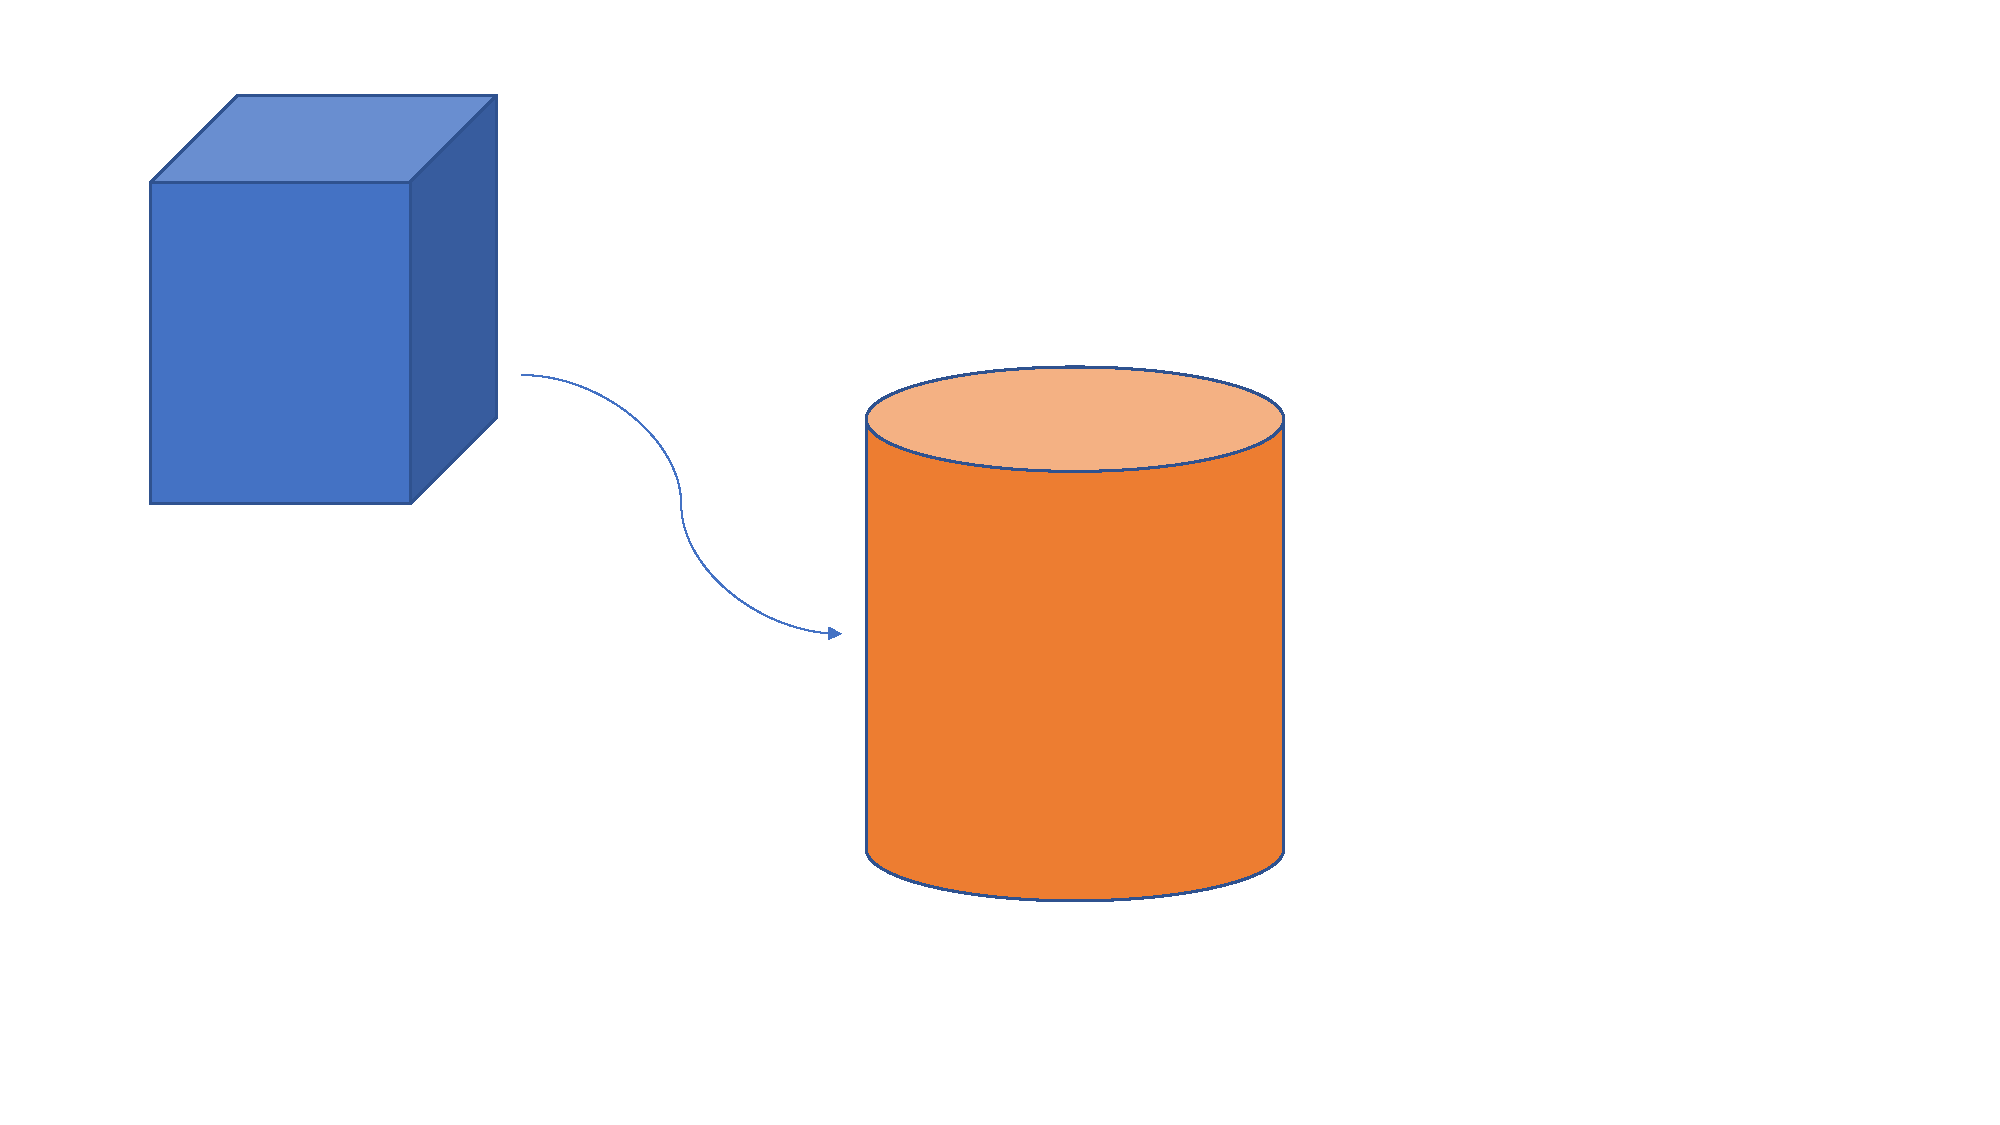
\includegraphics[width=0.80\textwidth]{a_Imagen01}
\caption{Donec vehicula augue eu neque.}
\label{fig:01_Proceso}
\end{figure}

\lipsum[2]


%%%%%%%%%%%%%%%%%%%%%%%%%%%%%%%%%%%%%%%%%%%%%%%%%%%%%%%%%%%%
\section{Ejemplo Link}
\lipsum[3-4]
En el \href{https://es.wikipedia.org/wiki/Proceso_(ingenier%C3%ADa)}{Wikipedia - Proceso} se pueden consultar la descripción
del proceso mostrado en la Figura~\ref{fig:01_Proceso}. 
